\subsection{Precisión versus rendimiento}
\label{subsec:resultados2}

\subsubsection{Introducción}

Al analizar nuestra implementación del blur gaussiano en busca de una posible
mejora o variante que pudiera resultar de interés, surgió la idea de cambiar el
tipo de dato en el que se procesaba la imagen. La versión de control utiliza
el tipo float lo cual asegura suficiente precisión al hacer los cálculos, pero a
veces esta precisión no es necesaria y se prefiere un rendimiento mayor en
términos de tiempos de ejecución. Es así como se nos ocurrió estudiar con más
detalle este camino y sus consecuencias.

Para los siguientes experimentos, se utilizó la implementación explicada en la
sección \ref{sec:blur_imp_exp}.

\subsubsection{Hipótesis}

A partir de las ideas mencionadas surgen varios experimentos para intentar
corroborar esta intuición acerca de cómo al sacrificar precisión podemos
posiblemente obtener un filtro de mayor velocidad.

Para empezar, tenemos que al pasar de punto flotante a enteros, dejamos de
tener que realizar conversiones de tipo y realizamos todas operaciones sobre
enteros, que en un principio deberían ser menos costosas que las de punto
flotante. Para esto la primer implementación de prueba que se realizó, difiere
con la de control únicamente en que en lugar de trabajar con floats, lo hace con
enteros de 32 bits, por lo cual procesa la misma cantidad de pixeles en
simultáneo, pero lo hace con instrucciones para enteros.

Por otro lado, si en nuestra versión de control trabajando con floats de 32 bits
operábamos de a un pixel a la vez, con nuestra implementación que utiliza
unsigned short de 16 bits estaríamos procesando dos pixeles en
simultáneo, llevándonos a suponer que esto nos brindaría una disminución en el
tiempo de ejecución a la mitad.

En ambos casos, además de observar los tiempos de ejecución, al bajar la
precisión suponemos que el cambio en la imagen resultante será proporcional a
cuanta precisión decidamos sacrificar.

\subsubsection{Experimentos}

Para corroborar nuestra hipótesis generamos un conjunto de imágenes cuadradas
con pixels de colores seleccionados de forma pseudo-aleatoria, para esto
realizamos el script \textit{random\_images\_generayor.py} que además tiene una semilla
la cual nos permite repetir el experimento con los mismos resultados. Este
conjunto de imágenes nos es útil en particular para analizar las diferencias
entre las imágenes resultantes de la implementación de control y la
experimental.

A partir de esto creamos imágenes de 5 tamaños distintos, que van de 25x25
hasta 400x400. Luego aplicamos a cada imagen el filtro la cantidad de veces
suficiente como para disminuir la varianza a un rango razonable. Una vez obtenidos estos
resultados analizamos qué tanto bajó la calidad de la imagen, para lo cual
generaremos una imagen con la intención de ver si a simple vista uno puede
diferenciar entre una versión con más precisión que otra.

Para comparar los resultados de los experimentos utilizamos las implementaciones
en ASM explicadas en la sección \ref{sec:blur_imp}. Nos referiremos a las mismas
de la siguiente forma:

\begin{itemize}
	\item \textbf{blur\_control}
		Versión de control, implementación de punto flotante. Procesa un pixel a
		la vez.
	\item \textbf{blur\_uint}
		Primer versión experimental, trabajando con enteros sin signo de 32 bit en lugar
		de números de punto flotante. Procesa un pixel a la vez.
	\item \textbf{blur\_ushort}
		Segunda versión experimental operando con enteros sin signo de 16 bit
		que le permiten procesar de a dos pixeles a la vez.
\end{itemize}

\subsubsection{Resultados y análisis}

A continuación se muestran los gráficos de rendimiento en términos de tiempo de
ejecución sobre las implementaciones mencionadas.

\begin{figure}[H]
	\centering
	\begin{minipage}{.5\textwidth}
		\centering
		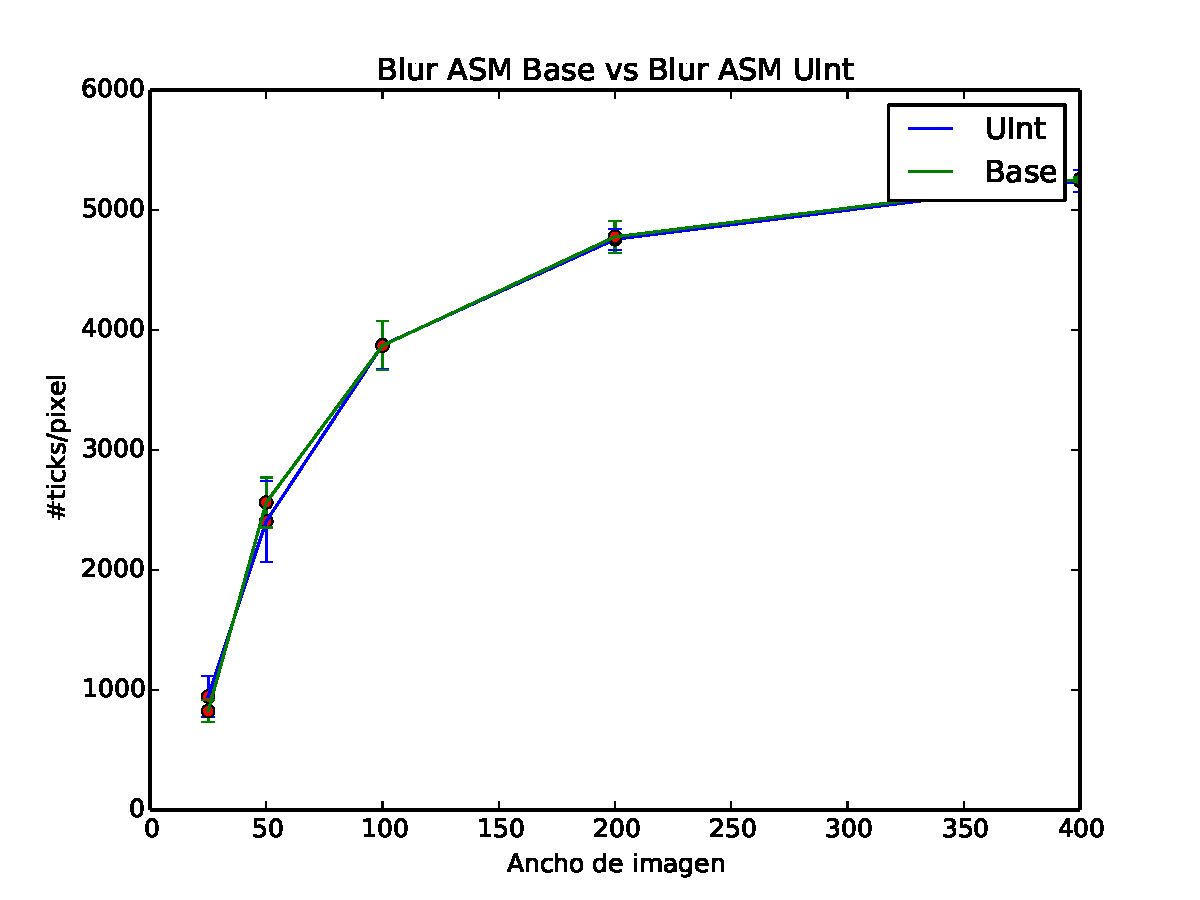
\includegraphics[width=\linewidth]{../graficos/blur_uint.pdf}
		\caption{\textbf{blur\_control} vs \textbf{blur\_uint}}
		\label{fig:blur_uint}
	\end{minipage}\hfill
	\begin{minipage}{.5\textwidth}
		\centering
		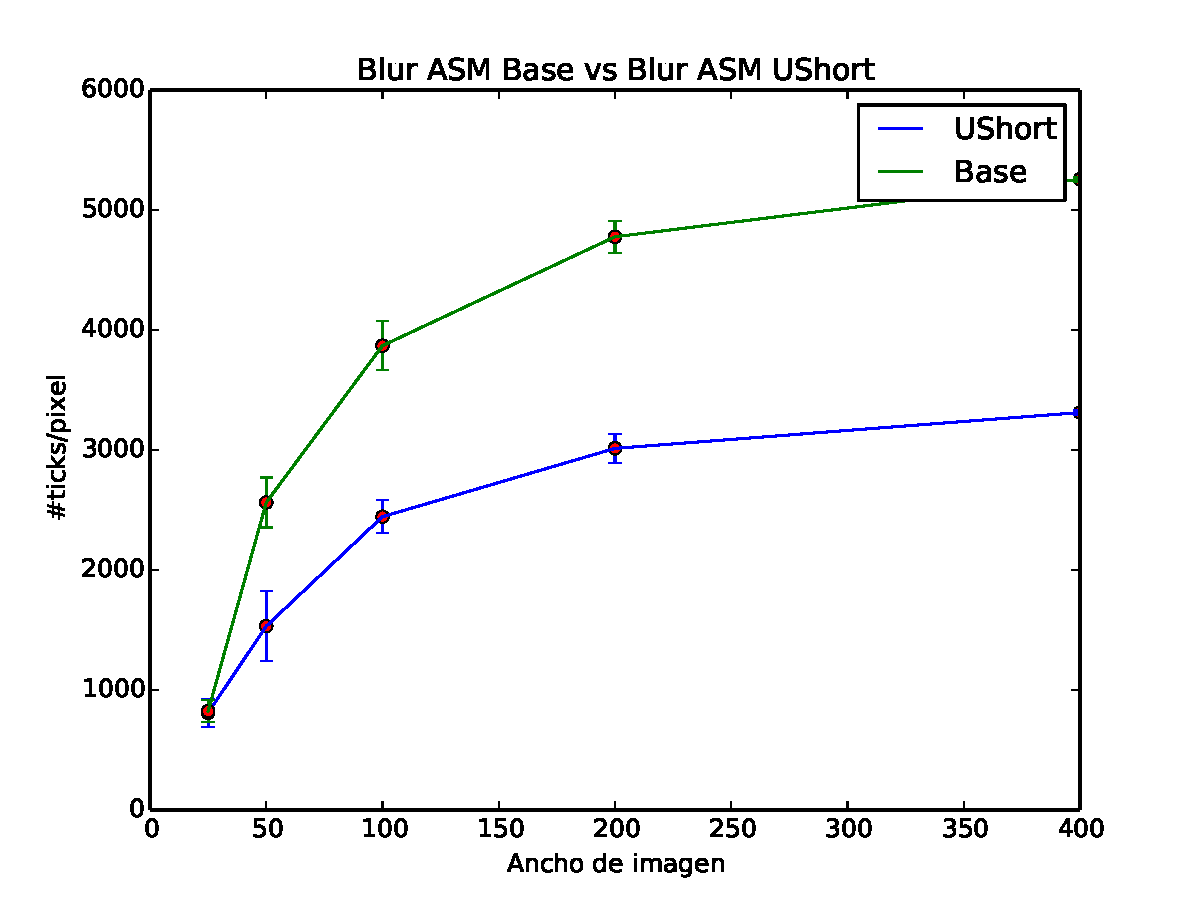
\includegraphics[width=\linewidth]{../graficos/blur_ushort.pdf}
		\caption{\textbf{blur\_control} vs \textbf{blur\_ushort}}
		\label{fig:blur_ushort}
	\end{minipage}
\end{figure}

Comencemos con la Figura \ref{fig:blur_uint}. Asumimos que al trabajar con enteros, al
evitar conversiones de tipo y operaciones de punto flotante se vería algún tipo
de mejora en tiempo de ejecución. Sin embargo, nos encontramos con que no se
çpresentó ningún tipo de mejora apreciable respecto la implementación de control,
por lo tanto una posible conclusión sería que las operaciones de conversión de
tipo y de punto flotante no agregan un costo apreciable.

Ahora si observamos la Figura \ref{fig:blur_ushort} tenemos un análisis mucho
más acertado. Aquí tenemos que la implementación \textbf{blur\_ushort} llega a
procesar al menos un tercio más rápido que \textbf{blur\_control}, corroborando
nuestra hipótesis que planteaba que el rendimiento aumentaría en cierta manera
proporcional a cuántos pixeles uno era capaz de procesar en simultáneo.

A continuación tenemos el resultado visual de estas tres versiones, donde
podemos analizar qué tanto influye en nuestra imagen final el sacrificio de
precisión.

\begin{figure}[H]
	\centering
	\begin{minipage}{.3\textwidth}
		\centering
		
\includegraphics[width=\linewidth]{imgs/chip_hd_v1.jpg}
		\caption{\textbf{blur\_control}}
		\label{fig:blur_prec_control}
	\end{minipage}\hfill
	\begin{minipage}{.3\textwidth}
		\centering
		
\includegraphics[width=\linewidth]{imgs/chip_hd_v1.jpg}
		\caption{\textbf{blur\_uint}}
		\label{fig:blur_prec_uint}
	\end{minipage}\hfill
	\begin{minipage}{.3\textwidth}
		\centering
		
\includegraphics[width=\linewidth]{imgs/chip_hd_ushort.jpg}
		\caption{\textbf{blur\_ushort}}
		\label{fig:blur_prec_ushort}
	\end{minipage}
	\caption*{Las tres figuras fueron producidas con $\sigma = 3$ y $r = 9$}
\end{figure}

Aquí tenemos otro punto de control, y se puede observar que hay una fuerte
relación entre la precisión que se maneja y nuestro resultado final. Para
\textbf{blur\_uint} la diferencia con respecto a \textbf{blur\_control} es
imperceptible al ojo humano, ya que esta versión trabaja con más precisión que
\textbf{blur\_ushort}. Por el otro lado, \textbf{blur\_ushort} para estos
parámetros terminó oscureciendo la imagen, lo que nos hace suponer que al
reducir tanto la precisión, lo más probable es que un número pequeño lo hubiera
redondeado a 0, resultando en que la matriz de convolución se aleje más a
integrar a 1 como observamos en la sección \ref{sec:blur_desc}.
